\chapter{Nutzenanalyse \& Business Case}

Ein Business Case (BC) ist eine Entscheidungsvorlage (Will man das Projekt durchführen?) für ein Vorhaben, die eine sachliche und eine betriebswirtschaftliche Begründung für das Vorhaben liefert. Ein Business Case besteht daher grob aus zwei Teilen:
\begin{enumerate}
	\item Sachliche (\emph{qualitative}) Begründung des Vorhabens. Prosa, braucht es immer, ca. 1 Seite.
	\item Wirtschaftliche (\emph{quantitative}) Begründung des Vorhabens. Zahlen, nicht immer, da zum Teil extrem aufwendig.
\end{enumerate}
Anhand des Business Cases werden die Projekte innerhalb des Projektportfolios priorisiert und evtl. auch gestrichen. Um verschiedene Projekte miteinander zu vergleichen, müssen für jedes einzelne davon Kosten und Nutzen quantitativ gegenübergestellt werden, auch wenn das nicht immer einfach ist. Abbildung \ref{fig:gliederung-business-case} zeigt eine typische Gliederung eines Business Cases.

\begin{figure}[h!]
\centering
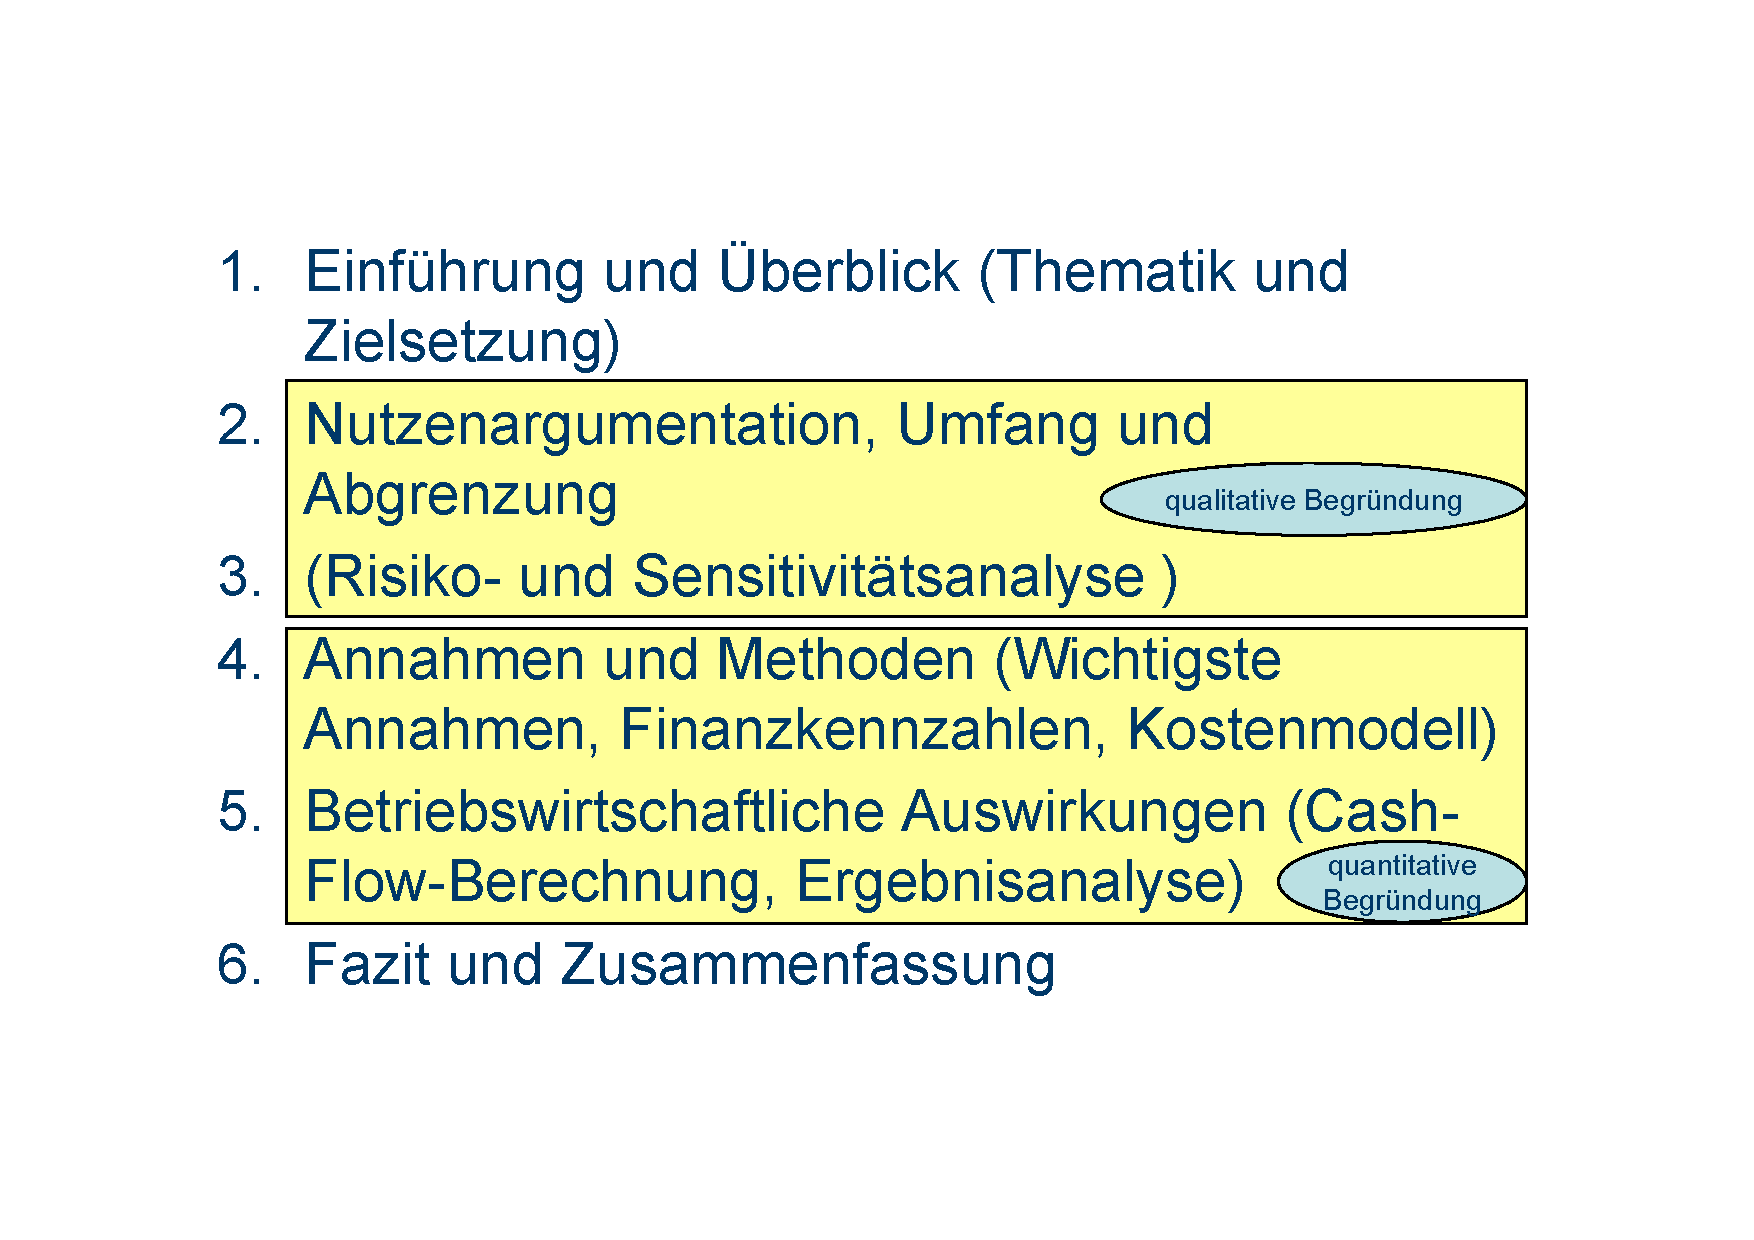
\includegraphics[width=0.7\linewidth]{fig/gliederung-business-case}
\caption{Typische Gliederung eines Business Cases}
\label{fig:gliederung-business-case}
\end{figure}

\section{Sie können die Hauptkostenarten des Total Cost of Ownership (TCO) für IT-Systeme angeben und erläutern.}

Die wichtigsten Kosten eines IT-Systems sind:
\begin{enumerate}
	\item Interne Personalkosten
	\item Externe Kosten (Personal und Dienstleistungen)
	\item Infrastrukturkosten (Räume, Rechner, Computernetzwerke, Hardware)
	\item Software- bzw. Lizenzkosten
\end{enumerate}
Bei den externen Personalkosten geht Geld aus der Firma raus deshalb werden externe und interne Personalkosten unterschieden. Anmerkung A. Kurmann: Interne Mitarbeiter muss man sowieso zahlen - ''funny money''.

\section{Sie können die Hauptnutzenarten für IT-Systeme angeben und erläutern.}

Der Nutzen eines IT-Systems lassen sich immer auf diese drei Arten herunterbrechen:
\begin{enumerate}
	\item Vorgaben (z. B. gesetzliche Bestimmungen) erfüllen (Pseudo-Nutzen)
	\item Kostenersparnis durch Effizienz Steigerung
    \item Zusätzliche/höhere Einnahmen (Umsatz steigern)
\end{enumerate}

Für eine Vorgabe braucht es in der Regel kein Business Case. Denn man muss es ja sowieso umsetzen. Hat man jedoch mehrere mögliche Lösungsvarianten lohnt es sich Business Cases für diese durchzurechnen.

\section{Die Studierenden können einen einfachen Business Case qualitativ beschreiben.}

Um einen Business Case qualitativ beschreiben zu können braucht man gute Kenntnisse der Materie. Es gibt auch einfache Beschreibungen, wenn z.B. eine gesetzliche Vorgabe erfüllt werden muss besteht der Business Case manchmal nur aus einem Satz. Ein solches Projekt kann nur oberste Priorität haben.
Wenn eine neue Geschäftsidee umgesetzt werden soll, kann der quantitative Teil eines Business Case entfallen. Meist fehlt noch die Erfahrung in diesem neuen Umfeld und man geht das Risiko bewusst in ein, um neues Geschäftspotenzial zu nutzen.

\section{Die Studierenden können einen einfachen Business Case quantitativ beschreiben, d. h. durchrechnen.}

Bei der quantitativen Seite braucht man noch tieferes Wissen der betroffenen Gebiete, um ein realistisches Budget zu erstellen. Eine Methode zur Berechnung von Kosten und Nutzen ist die Kapitalwertmethode. Bei der Kapitalwertmethode werden alle zukünftigen Erträge (Cash Flow) auf das Jahr der Investition zurückgerechnet und mit der Investition verglichen. Die zurückgerechneten Cash Flows werden auch \emph{Net Present Value} gennant und werden nach folgender Formel berechnet: $NPV=\frac{CF}{(1+i)^n}$. Abbildung \ref{fig:kapitalwertmethode} zeigt ein Beispiel wie geprüft werden kann ob sich eine Investition lohnt.

Im Business Case muss auch rein wie hoch die IT-Betriebskosten sind für die neue Lösung.

\begin{figure}[h!]
\centering
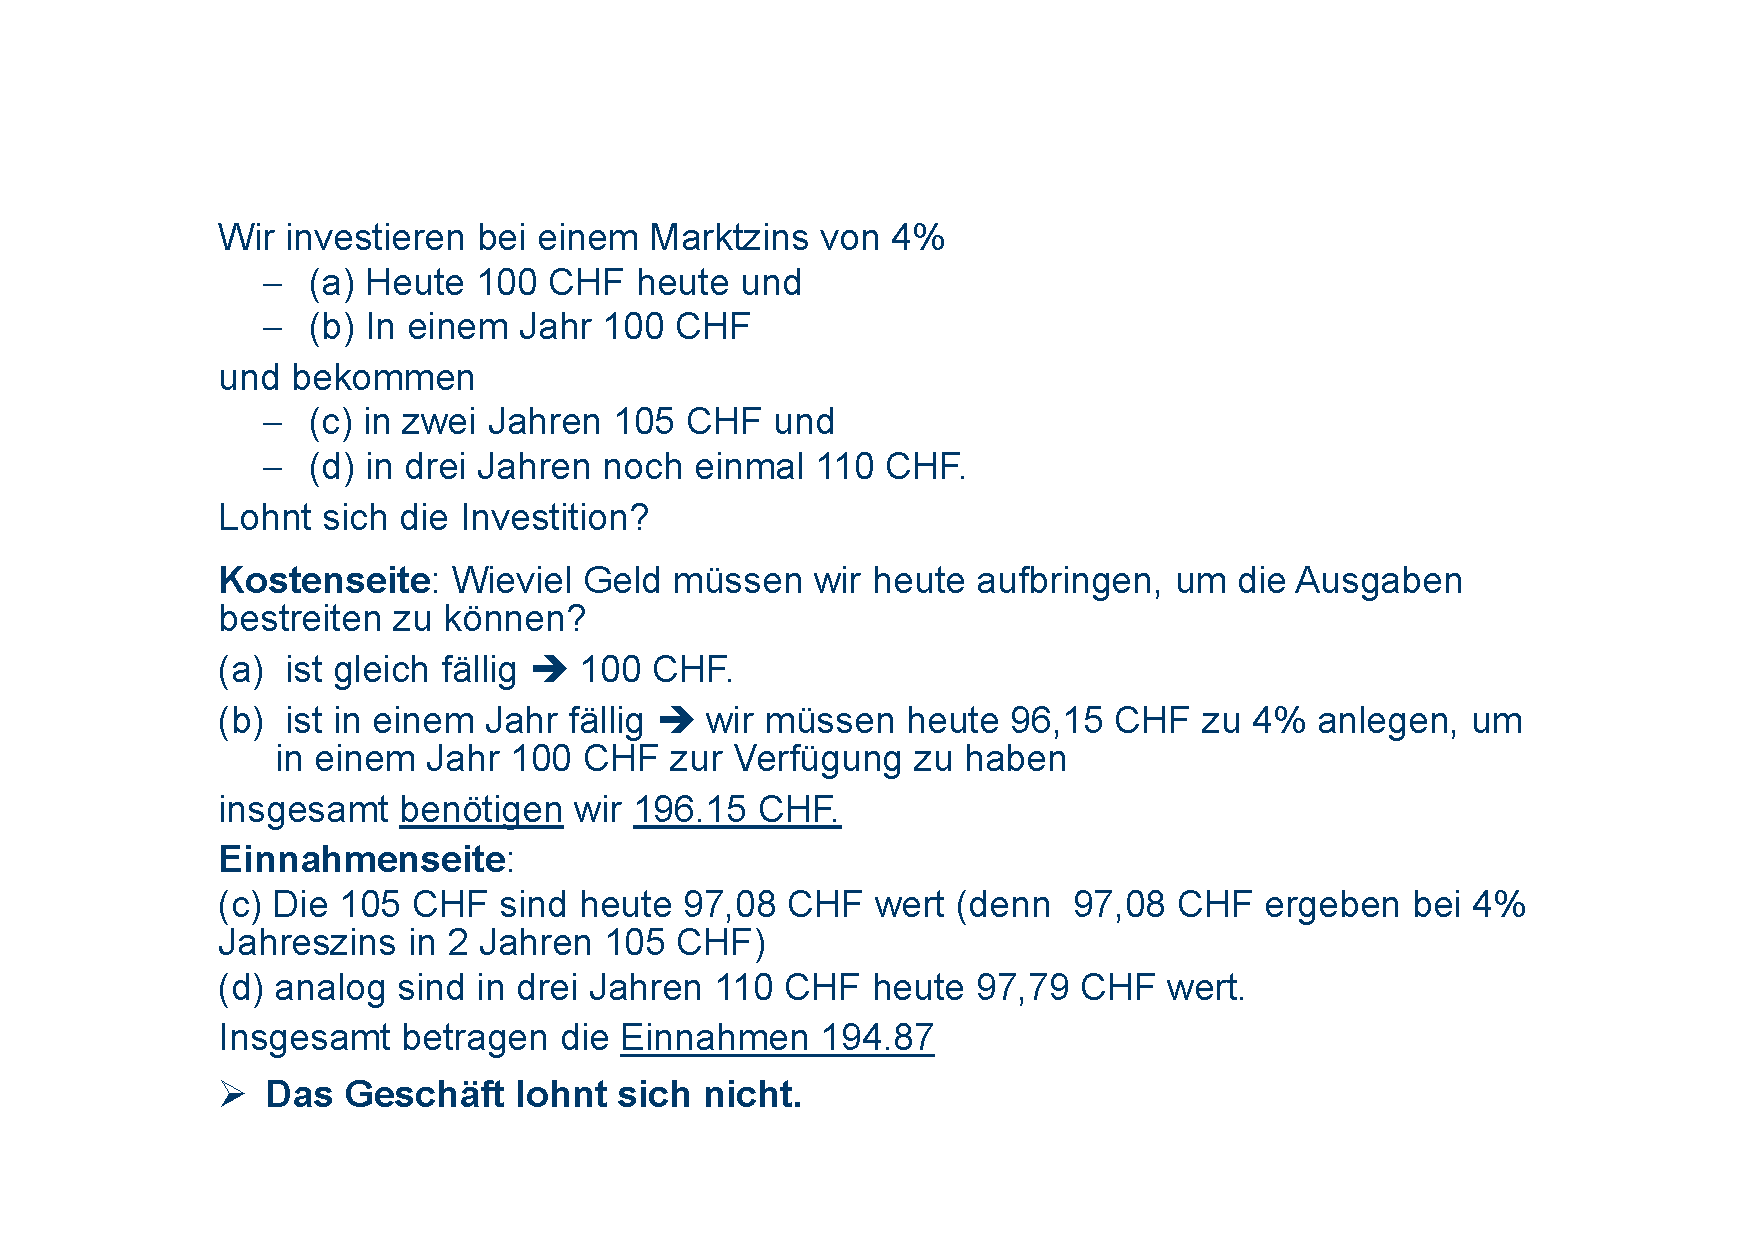
\includegraphics[width=0.8\linewidth]{fig/kapitalwertmethode}
\caption{Beispiel Kapitalwertmethode}
\label{fig:kapitalwertmethode}
\end{figure}

\section{Zusätzliche Fragen u. Antworten zur BC Fallstudie}
\subsection{Was ist ein Einkauf-Content?}
Ein Rückversicherer muss Daten einkaufen. Beispielsweise Börsendaten, Firmendaten usw. Ein Provider ist bspw. Reuters.

\subsection{Nutzenverteilung}
Beispielsweise sagt man, dass das Projekt im ersten Jahr nur 50 Prozent vom Nutzen abwirft, im zweiten 70 Prozent und erst im dritten 100 Prozent. So darf man beim Berechnen des Business Case im ersten Jahr nur 50 Prozent des Nutzen anrechnen.

\subsection{NPV}
Zahlungen über Jahre kann man nicht einfach so vergleichen. Man muss Zahlungen ''abzinsen'' und erhält somit den entsprechenden Kapitalwert (NPV). Denke da beispielsweise an die Inflation oder daran, dass man das Geld in andere Projekte investieren könnte. Bei der Berechnung gibt es zwei wichtige Zahlen:
\begin{description}
	\item[Anzahl Jahre] Über wie viele Jahre man den Business Case rechnet
	\item[Diskontsatz] Muss im gesamten Unternehmen einheitlich sein! Dies ist der Prozentsatz, welcher vorgegeben wird, mit welchem man abzinsen muss.
\end{description}

Der Projektleiter ist bestrebt diese zwei Variablen möglichst tief zu halten.

Im ersten Jahr, sprich das 0te-Jahr, ist die Potenz n = 0. Das ergibt einen Divisor von eins. Dies ist auch logisch. Wir haben im ersten Jahr keine Diskontierung!

Berechnung im BC: Man rechnet Ausgaben und Einnahmen pro Jahr aus. Das Resultat zinst man dann ab. Resultat / ((1 + Diskontsatz) \^ Anzahl Jahre)

Diskontierung bedeutet nichts anders als abzinsen. Man möchte den Wert einer zukünftigen Zahl für einen Zeitpunkt davor bestimmen.